\documentclass[twocolumn,11pt]{article}

\textheight 9 in
\voffset -.75 in

\usepackage{amssymb}
\usepackage{amsmath}
\usepackage{graphicx}
\usepackage{epstopdf}
\usepackage{tikz}
\usepackage{fancyhdr}
\usepackage{algpseudocode}
\usepackage{algorithm}
\usepackage[toc,page]{appendix}
\usepackage{url}

\setlength{\parskip}{5pt plus1pt minus1pt}

\DeclareMathSizes{36}{36}{36}{36}

\title{Train Harder, Smarter:\\Using Graph Theory to Create Route Suggestions}
\author{Forest Trimble\\trimbf@rpi.edu}
\begin{document}

\setlength{\headheight}{15pt}

\pagestyle{fancy}
\fancyhead{}
\fancyhead[L]{Forest Trimble}
\fancyhead[R]{Train Harder, Smarter}
\maketitle

\begin{abstract}
  \emph{Cyclists are always in search of the perfect ride on the perfect
  roads. They have criteria like distance and elevation gain to ensure
  that they get in the workout that they want. Unfortunately, to
  find this ideal ride manually, it takes a great deal of exploring and
  time, and eventually, one may settle into the habit of using the same
  roads that he/she already knows. We research a way to improve this
  paradigm, and to generate cyclists exactly the route they are looking
  for, without them having to do any work.}
\end{abstract}

\section{Background}

Cycling can be wildly different based on the roads that one takes: On busy
roads with no shoulders, it can be borderline miserable, while few things in
the world are better than spinning down a smoothly paved road with beautiful
vistas of open countryside and no traffic. Unfortunately, cyclists need to
invest massive amounts of time and energy exploring the roads and amassing a
repertoire that they can use. Additionally, it is difficult to satisfy criteria
for training, like an elevation gain and distance, using only that mental
repertoire. This paper chronicles the attempt to unroll a solution for this
problem.

Specifically, a good solution should take as input a distance to travel, a
start point, and, optionally, an elevation gain, and generate a route from the
start point that satisfies the distance and elevation gain within some
tolerance. A fully robust solution would also utilize user data to ensure that
it traverses the most pleasant roads to ride on and avoids the worst.

\section{Tools}

Creating a solution to this problem from scratch is unnecessary. The larger part
of this problem has already been solved: maps have been digitized and
parsers for the data format already exist. This section details the various
tools and technologies that the algorithm leverages.

First and foremost, we opted to use the Open Street Map format, which is open
source, fairly robust, and has a very active community that contributes to both
the maps themselves and to various (mostly open-source) software projects that
utilize the format. More information on this format can be found on their
website, openstreetmap.org.

Additionally, we leveraged some existing code to more easily be able to create
a demonstrable algorithm. Pyroute was used, since it has the very nice feature
that the navigation component was entirely decoupled into PyrouteLib. This
allows easy utilization of the Pyroute tools for GUI setup and OSM download
while also making it rather explicit where the navigation functions are. The
OSM wiki pages have a good deal of information
on Pyroute and PyrouteLib; refer to them for more information.

\section{Algorithm}

The core idea of our algorithm
is that at any point along the route, the engine generates weights for each
different possible direction to take, generates a random number, and picks a
direction according to the random number and the weights. There are several
different ideas that are competing for weight, so we'll break it down into the
individual components first, and then describe the combination at the end.

Additionally, the algorithm requires a few inputs from the user (in addition
to the Open Street Map network of roads):
\begin{itemize}
\item A distance to travel, $d$.
\item A direction in which to head $\phi$.
\item An elevation to gain, $h$.
\item A start point, $x_0$.
\end{itemize}

\subsection{Weight for Distance}

\begin{figure}
  \centering
  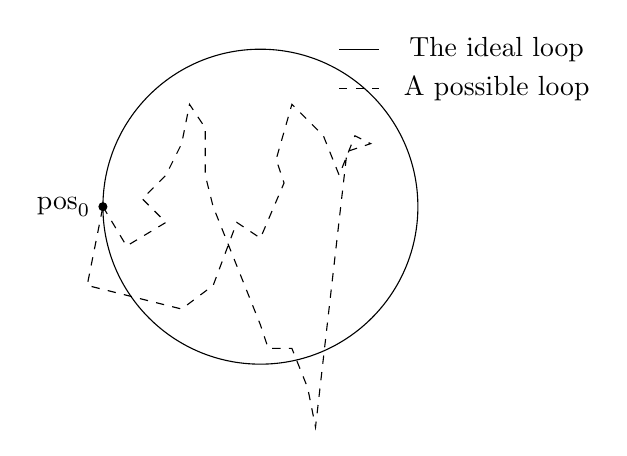
\begin{tikzpicture}
    \node (init) at (-0.5,0) {$\mbox{pos}_0$};
    \filldraw (0,0) circle(0.05);

    \draw (2,0) circle(2);
    \draw[dashed] (0,0) -- (0.3,-.5) -- (0.8,-0.2) -- (0.5,0.1) -- (0.8,0.4) --
    (1.0,0.8) -- (1.1,1.3) -- (1.3,1.0) -- (1.3,0.4) -- (1.4, 0) -- (1.6, -0.5)
    -- (1.8, -1) -- (2.0,-1.5) -- (2.1,-1.8) -- (2.4,-1.8) -- (2.6,-2.3) --
    (2.7,-2.8) -- (3.1,0.7) -- (3.4,0.8) -- (3.2,0.9) -- (3.0,0.4) -- (2.8,0.9)
    -- (2.4,1.3) -- (2.2,0.6) -- (2.3,0.3) -- (2.0,-0.4) -- (1.7, -0.2) --
    (1.4,-1) -- (1.0,-1.3) -- (-0.2,-1) -- (0,0);

    \node (mainleg) at (5,2) {The ideal loop};
    \node (altleg) at (5,1.5) {A possible loop};
    \draw (3,2) -- (3.5,2);
    \draw[dashed] (3,1.5) -- (3.5,1.5);
  \end{tikzpicture}
  \caption{The ideal loop starting at $\mbox{pos}_0$ contrasted with a possible
    actual loop} \label{fig:ideal}
\end{figure}

The first weight is based on distance. The idea is that there is a theoretical,
perfect loop that covers exactly the amount of distance that you would like,
and the algorithm does its best to direct you along that loop. See
Figure~\ref{fig:ideal} for an example of what this might look like.

\begin{figure}
  \centering
  \begin{tikzpicture}
    \node (theta) at (0,4.2) {$\theta$};


    \node (max) at (0.2,3) {2};
    \node (min) at (0.35,1) {0.5};
    \node (avg1) at (-1,2.2) {1};
    \node (avg2) at (1,2.2) {1};

    \draw[thick,<->] (0,0) -- (0,4);
    \draw[thick,<->] (-2,2) -- (2,2);
  \end{tikzpicture}
  \caption{A possible weighted compass} \label{fig:weights}
\end{figure}

In order to direct you along this loop, weights are generated based on
direction. We'll consider the method for finding the optimal direction,
$\theta$, briefly. First, consider how the weights are generated once
that direction is discovered. Basically, there is a weighted compass oriented
along $\theta$, with weights from 0.5 to 2. See Figure~\ref{fig:weights} to
see what we mean. As shown, the weights do not scale linearly. Instead, they
scale exponentially. This ensures that the weights are mostly centered around
the perpendicular, with growth accelerating farther from the perpendicular.
The idea is to have the weight be double in the ideal
direction, half moving exactly opposite the ideal direction, and unchanged
perpendicular to the ideal direction. Considering these three pieces of
information, we are looking for some $f : [0,2\pi] \to [0.5,2]$ as follows:
\begin{align*}
  2 = & f(\theta) \\
  1 = & f(\theta \pm \frac{\pi}{2}) \\
  \frac{1}{2} = & f(\theta \pm \pi)
\end{align*}
Let $\tau$ be the angle under consideration. We let
\[ \mbox{ang}(\tau, \theta) = |\theta - \tau \mbox{ mod } \pi|. \]
This allows us to define $f$ in terms of the angle between $\tau$ and
$\theta$. This function is necessary because $\theta$ is not necessarily
0. Note that this function only allows $\mbox{ang}(\tau, \theta)
\in [0,\pi]$. We accept this since we would like a compass symmetric
over the angle $\theta$, and we don't care if the angles are negative
or positive. However, the original function was defined in terms of the
value of $\tau$; instead, we are interested in a function based on the
angle between $\tau$ and $\theta$, which requires a slight redefinition:
\begin{align*}
  2 = & g(0) \\
  1 = & g(\frac{\pi}{2}) \\
  \frac{1}{2} = & g(\pi)
\end{align*}
We've already expressed the fact that we're interested in an exponential
function, and a base of two seems the obvious choice, leading to another
reduction:
\begin{align*}
  2 = 2^{h(0)} & \to & h(0) = 1 \\
  1 = 2^{h(\frac{\pi}{2})} & \to & h(\frac{\pi}{2}) = 0\\
  \frac{1}{2} = 2^{h(\pi)} & \to & h(\pi) = -1
\end{align*}
This yields two sets of three collinear points, which is easy enough to
map one to the other. Consider $h : [0,\pi] \to [-1,1]$ as follows:
\[ h(\mbox{ang}(\tau,\theta)) = 1 - \frac{2}{\pi}\mbox{ang}(\tau, \theta). \]
This satisfies the three points we gave, so we plug it in and calculate weight
accordingly:
\begin{equation}
  \mbox{WEIGHT} = 2^{1-\frac{2}{\pi}\mbox{ang}(\tau,\theta)}. \label{eq:weight}
\end{equation}


Now, we consider the method for finding the ideal direction. The idea behind the
direction loop is that if we had an ideal route, it would run exactly along that
path. Then the ideal direction is the one that puts us in the correct location
along that loop. First, consider how the loop is derived. It is a perfect
circle, passing through $x_0$, with a circumfrence of $d$, oriented according to
$\phi$. Note that $d$ and $x_0$ are fairly easy to understand, but the meaning
 of $\phi$ is less obvious. In order to understand what we mean, first consider
the parametric equations for a circle:
\[ x = \cos t \]
\[ y = \sin t \]
These equations generate the unit circle around the origin, something that we
will address later. For now, we are concerned only about what they mean for
$\phi$. Note that without alteration these equations will generate a
west-oriented loop: the circle starts at the rightmost point and proceeds left.
Consider a revised set of equations incorporating $\phi$:
\[ x = \cos (t + \phi) \]
\[ y = \sin (t + \phi). \]
As mentioned already, $\phi = 0$ corresponds to the west-oriented loop, and one
can quickly see that $\phi = \frac{\pi}{2}$ corresponds to the southern loop,
$\phi = \pi$ to the eastern, and $\phi = \frac{3\pi}{2}$ to the northern. That
being said, none of these loops actually start at the proper point; they are
centered around the origin rather than beginning at it. In order to have any
choice of $\phi$ generate a loop that starts at the origin, we can simply zero
out the initial value:
\[ x = \cos (t + \phi) - \cos \phi \]
\[ y = \sin ( t + \phi ) - \sin \phi. \]
This gives a much more obvious representation of our ideal loop, which starts
at (0,0), and traces out a loop according to $\phi$. One thing of interest is
that $\phi$ is exactly $\pi$ plus the compass direction that we would expect.

Once you recall that our distance goal, $d$, is the circumfrence of the loop,
it is easy to see that the radius is $\frac{d}{2\pi}$. We can then adjust our
equation to correspond with our starting point and radius as follows:
\[ x = \frac{d}{2\pi}(\cos ( t + \phi ) - \cos \phi ) + x_0 \]
\[ y = \frac{d}{2\pi}(\cos ( t + \phi ) - \cos \phi ) + y_0 \]
Of course, this needs some adjustment to deal with the difference of using
latitude and longitude over a cartesian coordinate system, since latitude
and longitude are not actually coordinates on a 2-d plane, but rather angles
that are made against the center of the Earth. For now, this is sufficient to
get an idea of what is happening, but we'll cover how this will be converted
into a latitude/longitude format in Section~\ref{sec:latlong}.

Until now, we've used $t$ to represent the angle in the parametric equation,
without delving into what it really means. However, we can use a much more
useful expression to represent this angle: $\frac{2\pi}{d}d_i$, where $d_i$ is
the current distance travelled, gives us the
angle in terms of a percentage of the requisite distance travelled. This gives
us the advantage of knowing exactly where in the loop we should be at any
current distance travelled. This also needs to be capped after $d_i \geq d$.
Incorporating this yields the final equations:
\[ x = \frac{d}{2\pi}(\cos (\min(\frac{2\pi}{d}d_i,2\pi) + \phi) - \cos \phi) + x_0 \]
\[ y = \frac{d}{2\pi}(\sin (\min(\frac{2\pi}{d}d_i,2\pi) + \phi) - \sin \phi)+ y_0. \]

\begin{figure}
  \centering
  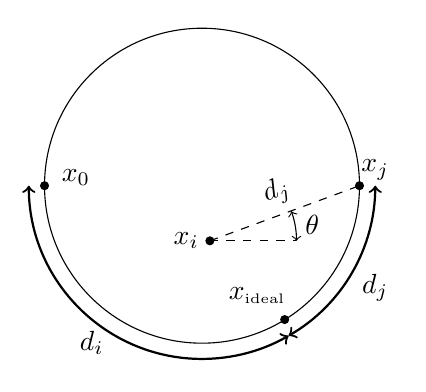
\begin{tikzpicture}
    \draw (2,0) circle(2);
    \filldraw (0,0) circle(0.05);
    \node at (0.4,0.1) {$x_0$};

    \draw[thick,<->] (-0.2,0) arc (180:300:2.2);
    \node at (0.6,-2) {$d_i$};
    \filldraw (3.05,-1.7) circle(0.05);

    \draw[thick,<->] (4.2,0) arc (0:-60:2.2);
    \node at (4.2,-1.3) {$d_j$};

    \filldraw (4,0) circle(0.05);
    \node at (4.2,0.2) {$x_j$};

    \node at (1.8,-0.7) {$x_i$};
    \node at (2.7,-1.4) {$x_{\mbox{{\tiny ideal}}}$};

    \filldraw (2.1,-0.7) circle (0.05);

    \draw[dashed] (2.1,-0.7) -- (4,0) node[above,midway,sloped] {$d_j$};

    \draw[dashed] (2.1,-0.7) -- (3.2,-0.7);
    \draw[<->] (3.2,-0.7) arc(0:20:1.1);
    \node at (3.4,-0.5) {$\theta$};
  \end{tikzpicture}
  \caption{Important values for the algorithm \emph{Note: not to scale}}
  \label{fig:algvals}
\end{figure}

The next step is to utilize these equations to calculate $\theta$. At any point
along the algorithm, we are at some $x_i$, and we have travelled a distance,
$d_i$. Figure~\ref{fig:algvals} should help to understand what exactly the
algorithm is attempting to achieve. The idea is this: if we have travelled some
distance $d_i$, then there is an $x_{\mbox{{\tiny ideal}}}$ on the ``ideal''
loop. The arc between $x_{\mbox{{\tiny ideal}}}$ and $x_0$ will be of length
$d_i$. The algorithm searches for a point $x_j$ such that the arc between
$x_{\mbox{{\tiny ideal}}}$ and $x_j$ will have the \emph{same} distance as the
line between $x_i$ and $x_j$. Fortunately, we have framed the equations for
calculating $x_j$ in terms of the distance travelled along the arc, and the
distance between $x_i$ and $x_j$ can easily be calculated using the pythagorean
theorem. Note that we find $x_j$ as follows:
\begin{align}
  x_j = \frac{d}{2\pi} ( & \cos( \frac{ 2 \pi }{ d } ( \min( d, d_i + d_j ) )
                                  + \phi ) \notag \\ & - \cos \phi ) + x_0
                                  \label{eq:xj} \\
  y_j = \frac{d}{2\pi} ( & \sin( \frac{ 2 \pi }{ d } ( \min( d, d_i + d_j ) )
                                  + \phi ) \notag \\ & - \sin \phi ) + y_0.
                                  \label{eq:yj}
\end{align}
To satisfy our constraint, we have
\[ d_j = \sqrt{ ( x_j(d_j) - x_i )^2 + ( x_j(d_j) - x_i )^2 }. \]

\subsubsection{Finding $d_j$}
Obviously, this is a rather difficult equation to truly solve, so we must only
heuristically find a solution. Unfortunately, even the heuristic solution is
a difficult one for a few reasons. Most problematically, the sine and cosine
functions have up to two stationary points on the interval we are considering
and there may not be a solution of $d_j$ that will satisfy the equality.
Nonetheless, we will do our best to mitigate these issues and apply a good
heuristic to find $d_j$. First, we rearrange our equation so that we can apply
a root-finding approximation algorithm to it:
\begin{equation}
  f(d_j) = \sqrt{(x_j(d_j) - x_i)^2 + (y_j(d_j) - y_i)^2} - d_j. \label{eq:dj}
\end{equation}
This simply allows the $d_j$ we are looking for to be the zero of the function.
The first exciting bit of news is that for most solutions of this equation with
$d_j < d$, it will work out that $f(0) > 0$ and $f(d-d_i) < 0$.
We know that $f(0) \geq 0$ by the
positivity of norms, and the square root of the sum of the squares is the
euclidian norm. We also can be certain that $f(d-d_i) < 0$ since
the norm is also unable to change by more than the diameter
of the ideal loop, or even less based on the proximity of $x_i$ to the center of
the loop. In situations where $f(d-d_i) > 0$, we notice that the distance to the
start of the loop is further away than the amount of distance we have left to
travel; this means that we should just route back to the start anyways. As such,
we have bounds inside of which we know that there exists a solution. We apply
Brent's method, a robust root approximation algorithm, to determine the solution
inside of this zone. The idea behind Brent's method is to combine the bisection
method, the secant method, and inverse quadratic interpolation. Readers
unfamiliar with any of these techniques should refer to CITATIONS. Some
pseudocode is given for Brent's Method in Algorithm~\ref{alg:brent}. The idea
is this:

First, we need a bracket in which our function has a root. For us, this is
simple enough; we just use $[0, d-d_i]$. If that bracket does not satisfy the
condition, we just set $d_j = d-d_i$ and don't bother with anything.

The algorithm details out the actual swapping of $a_k$ and $b_k$, but here
we'll just assume that $|f(a_k)| > |f(b_k)|$ at all points in time; that is,
$b_k$ is a better approximation of the solution than $a_k$. We also require
$b_{k-1}$; for now, we'll set it to $a_k$.

This is a heuristic, so we'll keep repeating the algorithm until either
$a_k \approx b_k$ or $f(b_k) \approx 0$. At the $k^{\mbox{{\tiny th}}}$ iteration,
we'll calculate $b_{k+1}$ using both inverse quadratic interpolation and the
bisection method.

In general, the inverse quadratic interpolation can proceed very quickly, but we
add the bisection method to ensure convergence. In using interpolation, one of
the following conditions must be satisfied:
\begin{itemize}
\item Inverse Quadratic Interpolation was performed last time,
  \[ |s - b_k| < \left|\frac{b_{k-1}-b_{k-2}}{2}\right|, \]
  and
  \[|\delta| < |b_{k-1} - b_{k-2}| \]
\item The Bisection Method was used last time,
  \[|s - b_k| < \left|\frac{b_k-b_{k-1}}{2}\right|, \]
  and
  \[ |\delta| < |b_k - b_{k-1}| \]
\end{itemize}
The rest of the pseudocode serves only to ensure that variables are assigned
correctly. One notes that mflag indicates whether interpolation was used last
time or not.

\begin{algorithm}
  \caption{Using Brent's Method to find a zero of a function}
  \label{alg:brent}
  \begin{algorithmic}
    \Require $f(a_0)f(b_0) > 0$
    \Function{Brent}{$f : [a,b] \to \mathbb{R}$, $a_0$, $b_0$}
      \If{$|f(a_0)| < |f(b_0)|$}
        \Call{swap}{$a_0$,$b_0$}
      \EndIf
      \State $b_{k-1} \gets a_0$
      \State mflag $\gets$ True
      \While{$f(b_k) \not = 0$ {\bf and} $|b_k - a_k| > \epsilon$}
      \begin{align*}
        s \gets &\frac{a_kf(b_k)f(b_{k-1})}{(f(a_k)-f(b_k))(f(a_k)-f(b_{k-1}))} \\
        & + \frac{b_kf(a_k)f(b_{k-1})}{(f(b_k)-f(a_k))(f(b_k)-f(b_{k-1}))} \\
        & + \frac{b_{k-1}f(a_k)f(b_k)}{(f(b_{k-1})-f(a_k))(f(b_{k-1})-f(b_k))}
      \end{align*}
      \State {\bf if} $\displaystyle s \not \in \left[ \frac{3a_k+b_k}{4},b_k \right]$
             {\bf or}
             \State ~~~~(mflag is True {\bf and}
             \State ~~~~~~~~ ($\displaystyle |s-b_k| \geq \frac{|b_k-b_{k-1}|}{2}$
             \State ~~~~~~~~~~ {\bf or} $|b_k-b_{k-1}| < |\delta|$)) {\bf or}
             \State ~~~~(mflag is False {\bf and}
             \State ~~~~~~~~ ($\displaystyle |s-b_k| \geq \frac{|b_{k-1}-b_{k-2}|}{2}$
             \State ~~~~~~~~~~ {\bf or} $|b_{k-1}-b_{k-2}| < |\delta|$)) {\bf then}
             \State ~~~~ $\displaystyle s \gets \frac{a_k+b_k}{2}$
             \State ~~~~ mflag $\gets$ True
             \State {\bf else}
             \State ~~~~ mflag $\gets$ False
        \State $b_{k-2} \gets b_{k-1}$
        \State $b_{k-1} \gets b_k$
        \If{$f(a_k)f(s) < 0$}
          \State $b_k \gets s$
        \Else
          \State $a_k \gets s$
        \EndIf
        \If{$|f(a_k)| < |f(b_k)|$}
          \Call{swap}{$a_k$,$b_k$}
        \EndIf
      \EndWhile
    \EndFunction
  \end{algorithmic}
\end{algorithm}

Thus, by utilizing Brent's Algorithm, we can find $x_j$. From here, calculating
$\theta$ is fairly straightforward:
\begin{align}
  \tan \theta = & \frac{y_j - y_i}{x_j-x_i} \notag \\
  \theta = & \tan^{-1} \frac{y_j - y_i}{x_j-x_i} \label{eq:theta}
\end{align}

Finally, we have a method for calculating the weights based on distance and
direction! Use Brent's algorithm as described in Algorithm~\ref{alg:brent}
with the function to be zeroed as \eqref{eq:dj}. Use that $d_j$ in conjunction
with \eqref{eq:xj} and \eqref{eq:yj} to find
$x_j$ and $y_j$, respectively, and plug into \eqref{eq:theta} to find a
$\theta$. Finally, use $\theta$ in conjunction with \eqref{eq:weight} to assign
weights to directions.

\subsection{Weight for Elevation Gain}

Now that weights have been assigned based on distance and direction, we can
move on to worrying about elevation gain.

FILL IN THIS SECTION

\subsection{Miscellaneous Weights}

There are a few more important characteristics to consider when calculating
weights. Perhaps the easiest of these to deal with are the built in road types
that the Open Street Map format provides. It is easy enough to assign these
priorities based on what a cyclist would reasonably hope to see. Basically,
busy roads get weighted lower than low-traffic roads, but things like
pedestrian walkways and other unridable roads also get high weights.

Another characteristic to consider is whether a road has already been
travelled. Repeatedly riding along the same stretch of road can make a ride
rather boring, so by weighting against this, it can be avoided.

\subsection{Using the Weights Together}

\section{Moving to Three Dimensions} \label{sec:latlong}

\section{Experimentation \& Results}

\section{Discussion}

\section{Future Work}

There are many ways to expand the algorithm developed here. While we have done
our best to utilize as much data as possible, expanding the set of data utilized
to generate the routes will likely improve the algorithm.


 (ASK DAN FOR THIS
PAPER) There has been research done into analyzing the probability of accidents
on a road based on certain metadata. This metadata is readily available to the
cities that own the roads, but it is seldom available for direct access inside
of maps. If this data becomes more readily available, then it can be integrated
into the application to help increase user safety.

Additionally, this has been a facet of a three pronged project developing a
platform for bicycle training. The other two aspects are developing an Android
application to track training data during a ride and a website to track
long-term training data. Ideally, this algorithm will eventually be seamlessly
integrated into the mobile and web projects, so that routes can be generated
and sent directly to the application for the user to follow.

Once the three prongs of this project have been integrated together, leveraging
the data from the other parts would also provide valuable input for the
algorithm. One of the most exciting applications of this information is to
generate something similar to a heatmap of roads that users of the website
ride. With this heatmap, the weights could be improved and generated based on
popularity.

Finally, it might be interesting to generate routes that are not necessarily
circuits. Loops are generally more useful since cyclists are likely to want
to return home after a good training ride, but it might also be useful to
have some sort of quasi-navigation that aims for the most fun route
between two locations rather than the most direct route.

\end{document}
